\section{Basics}

\begin{frame}
	\frametitle{Commitments}
	\framesubtitle{Introduction}
	\begin{columns}
		\begin{column}{0.5\textwidth}
			\begin{figure}
				\centering
				
\includegraphics[width=0.8\linewidth]{Images/lollipop}
				\caption{Kung Fu Hustle - Lollipop Girl}
				\label{fig:lollipop}
			\end{figure}
		\end{column}
		\begin{column}{0.5\textwidth}
			\begin{Large}
				Plot Summary:
				\begin{enumerate}
					\item Villain destroys village and steals girls lollipop
					\item Girls swears vengeance
					\item Girl becomes Kung Fu - master
					\item Girl finds the villain. Villain recognices her by the lollipop	
				\end{enumerate}
			\end{Large}
		\end{column}
	\end{columns}
\end{frame}

\begin{frame}
	\frametitle{Commitments}
	\framesubtitle{Basic-protocoll}
	\begin{columns}
		\begin{column}{0.5\textwidth}
			\begin{LARGE}
				\begin{itemize}
					\item A \textbf{commits} to B
					\item B keeps commitment, unable to read or process it
					\item A \textbf{reveals} to B
					\item B verifies the commitment 
				\end{itemize}
			\end{LARGE}
		\end{column}
		\begin{column}{0.5\textwidth}
			\begin{figure}
				\centering
				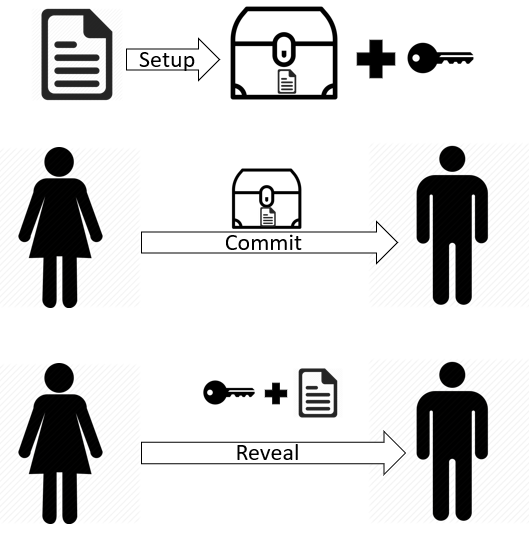
\includegraphics[width=0.8\linewidth]{Images/protocoll}
				\caption[Commitments]{Commitments}
				\label{fig:protocoll}
			\end{figure}
		\end{column}
	\end{columns}	
\end{frame}

\begin{frame}
	\frametitle{Commitments}
	\framesubtitle{Attributes}
	\begin{enumerate}
		\item \textbf{Binding:} The Values Alice put in the Commitment cannot be changed after B recieved it 
		\item \textbf{Hiding:} Bob cannot gain any information about the message from the commitment itself
		\item \textbf{Viability:} If both parties follow the Protocoll, Bob is always able to recover the committed value
	\end{enumerate}
	Additional for \textit{real-life-applications}:
	\begin{enumerate}
		\item Bobs are able compare commitments
		\item Commitments are \textit{tradeable} and replicable
	\end{enumerate}
\end{frame}

\begin{frame}
	\frametitle{Commitments}
	\framesubtitle{Applications}
	\begin{columns}
		\begin{column}{0.5\textwidth}
			\textbf{Challenge and Response} ~\newline
			You can setup your own anonymus challenges, leaving a commitment at Bob's. If someone show's up saying he's Alice, Bob challenges to reveal the commitment.
		\end{column}
		\begin{column}{0.5\textwidth}
			\textbf{JSON-Web-Tokens (JWT):} ~\newline
			A payload (e.g. some account details) are encrypted and linked to a commitment and passed to a third party. ~\newline 
			You can verify yourself at the third-party revealing the commitment ~\newline 
			this is done \textit{automatic} via session or systemattributes 
		\end{column}
	\end{columns}
\end{frame}